% easychair.tex,v 3.2 2012/05/15
%
% Select appropriate paper format in your document class as
% instructed by your conference organizers. Only withtimes
% and notimes can be used in proceedings created by EasyChair
%
% The available formats are 'letterpaper' and 'a4paper' with
% the former being the default if omitted as in the example
% below.
%
\documentclass{easychair}
%\documentclass[debug]{easychair}
%\documentclass[verbose]{easychair}
%\documentclass[notimes]{easychair}
%\documentclass[withtimes]{easychair}
%\documentclass[a4paper]{easychair}
%\documentclass[letterpaper]{easychair}

% This provides the \BibTeX macro
\usepackage{doc}
% \usepackage{makeidx}

% In order to save space or manage large tables or figures in a
% landcape-like text, you can use the rotating and pdflscape
% packages. Uncomment the desired from the below.
%
\usepackage{rotating}
% \usepackage{pdflscape}

\usepackage[ruled,vlined]{algorithm2e}
\DontPrintSemicolon

\usepackage{minibox}
\usepackage{caption}
\usepackage{multirow}
\usepackage{graphicx}
%\makeindex

%% Document
%%
\begin{document}

%% Front Matter
%%
% Regular title as in the article class.
%
\title{Efficient Graph Kernels for RDF data using Spark}

% \titlerunning{} has to be set to either the main title or its shorter
% version for the running heads. When processed by
% EasyChair, this command is mandatory: a document without \titlerunning
% will be rejected by EasyChair

\titlerunning{Efficient Graph Kernels for RDF data using Spark}

% Authors are joined by \and. Their affiliations are given by \inst, which indexes
% into the list defined using \institute
%
\author{
Bernhard Japes\inst{1}
\and
Shinho Kang\inst{2}
}

% Institutes for affiliations are also joined by \and,
\institute{
  Informatik III, Universit\"at Bonn,
  Germany\\
  \email{bernhard.japes@uni-bonn.de}
\and
   Informatik III, Universit\"at Bonn,
   Germany\\
   \email{TODO}\\
 }
%  \authorrunning{} has to be set for the shorter version of the authors' names;
% otherwise a warning will be rendered in the running heads. When processed by
% EasyChair, this command is mandatory: a document without \authorrunning
% will be rejected by EasyChair

\authorrunning{Bernhard and Shinho}


\clearpage

%%%%%%%%%%%%%%%%%%%%%%%%%%%%%%%%%%%%%%%%%%%%%%%%%%%
\maketitle
%%%%%%%%%%%%%%%%%%%%%%%%%%%%%%%%%%%%%%%%%%%%%%%%%%%

\begin{abstract}
In this paper we study the application of graph kernels for RDF data using the popular Apache Spark\footnote{http://spark.apache.org} engine in combination with the SANSA-Stack\footnote{http://www.sansa-stack.net} data flow utilities.
We focus on an implementation of the Intersection Tree Path (ITP) Kernel, published by Gerben Klaas Dirk de Vries and Steven de Rooij in \cite{FGK}, that is based on the concept of constructing a tree for each instance and counting the number of paths in that tree.
\end{abstract}

\setcounter{tocdepth}{2}
\pagestyle{empty}

%------------------------------------------------------------------------------
\section{Introduction}
\label{sect:Introduction}
The increasing availability of structured data and the rise of the semantic web pose new challenges for machine learning and data mining. As an official standard, the \textit{Resource Description Framework} (RDF) is commonly used to represent those graphs, which led to research on how to use the RDF structure to predict links and labels of instances efficiently. Most of the current approaches to mining structured graph-data focus on specific semantic properties and are individually designed for different problems \cite{Rettinger2009, Huang2011}.

Kernels, however, have already been proven to be useful as a much more flexible approach for Pattern Analysis in different areas \cite{Shawe-Taylor2004}, which resulted in further research on specific graph kernels for RDF. The main drawback of most of these graph kernels, including the state-of-the-art \textit{Weisfeiler-Lehman} (WL) RDF kernel, is their computation time as shown in \cite{deVries2013}. In \cite{FGK} Gerben Klaas Dirk de Vries and Steven de Rooij present a \textit{Fast and Simple Graph Kernel for RDF} with just a slightly worse prediction performance than the WL graph kernel, but the huge upside of being 10 times faster in practice. Their idea of a fast and simple, but scalable kernel also seems to be promising for big data applications. However several adaptions of their algorithm are required to ensure consistent computations on distributed data sets using the Apache Spark engine.

%------------------------------------------------------------------------------
\section{Approach}
\label{sect:Approach}

The graph kernel presented in \cite{FGK} is based on the idea that instances are represented by their subgraphs. This assumption implies that we should be able to explicitly compute a feature vector for each instance by constructing a tree, starting from the instance vertex up to a certain depth $d$, and counting the paths. Now taking the dot product of two feature vectors is essentially the intersection of both trees. The original pseudo-code for the so called Intersection Tree Path (ITP) Kernel is given in Algorithm 1.

\begin{algorithm}
 \label{alg:ITP}
 \KwData{a set of RDF triples $R$, a set of instances $I$ and a max depth $d_{max}$ }
 \KwResult{a set of feature vectors F corresponding to the instances I}
 \textbf{Comment:} $pathMap$ is a global map between paths of vertices and edges and integers\;
 \;
 - set $pathIdx = 1$\;
 - for each $i \in I$\; \Indp
 - create a new feature vector $fv$\;
 - do $processVertex(i,i,[],fv,d_{max})$\;
 - add $fv$ to $F$\; \Indm
 \;
 \textbf{function} $processVertex(v,root,path,fv,d)$\; \Indp
 - if $d = 0$, return \;
 - for each $(v,p,o) \in R$\; \Indp
 - if $o$ is $root$, set $path = [path,p,rootID]$\;
 - else, $path = [path, p, o]$\;
 - if $pathMap(path)$ is undifned\; \Indp
 - set $pathMap(path) = pathIdx$
 - set$pathIdx = pathIdx + 1$\; \Indm
 - set $fv(pathMap(path)) = fv(pathMap(path)) + 1$\;
 - do $processVertex(o,root,path,fv,d-1)$\;
\caption{The Intersection Tree Path (ITP) Kernel as introduced in \cite{FGK}}
\end{algorithm}

This algorithm can be directly applied to small and medium size datasets. However, big datasets are commonly distributed on different nodes as a \textit{Resilient Distributed Dataset} (RDD), or \textit{DataFrame} (DF) \cite{RDDpaper} and should be processed in parallel by using frameworks like Spark and SANSA. One main aspect of the ITP kernel is the iterative construction of paths and the associated $pathMap$ that assigns a unique integer to each path. To optimize the performance on distributed data we want to avoid this iterative and not parallelized construction if possible.

This can be achieved by using a different representation of the constructed trees as shown in algorithm 2. To keep track of the different \textit{Uniform Resource Identifiers} (URIs) of subjects and objects during the parallelized construction of trees, we start off by mapping these URIs iteratively to integers. Furthermore we map the instances to their respective label and transform the TripleRDD, generated by using the SANSA RDF utilities, to a DataFrame. Construction of the paths of trees is implemented as a series of SQL queries on DataFrames utilizing the inherent structure. Instead of representing each path as an integer on a $pathMap$, as in the ITP kernel, we construct each path in $pathDF$ as a \textit{String} containing the predicates and objects respectively subjects.

Based on all the paths created and stored in $pathDF$ we can now compute the trees by aggregating paths and collecting them as an Array[\textit{String}] for each subject. Now those Array[\textit{String}] can not only be interpreted as a tree in form of a list of paths, but also as a regular text document using paths as a vocabulary.  In doing so we can make use of the \textit{Spark ML CountVectorizer} that is designed to convert a collection of text documents to vectors of token counts, extracting the vocabulary in form of a sparse representation. This basically replaces the $pathMap$ with the huge upside of performing parallelized on distributed data. 

The Array[\textit{String}] of each subject is transformed to a sparse vector containing information which paths are part of the tree with a consistent mapping for all subjects covering all the occurring paths. These sparse vectors can be used as feature vectors for different machine learning algorithms of the \textit{Spark ML} and {MLlib} libraries like logistic regression or random forests.
\begin{algorithm}
 \label{alg:FTGK}
 \KwData{a TripleRDD $R$, an instance DF $I$ and a max depth $d_{max}$ }
 \KwResult{a set of feature vectors F corresponding to the instances I}
 \;
 \textbf{Initialization:}\; \Indp
 - map subjects and objects in $R$ and $I$ to unique integers\;
 - map instances in $I$ to their label\;
 - transform $R$ into a DF $T$ with columns ($s,p,o$) for subject, predicate and object\; \Indm
\; 
\textbf{Construct the paths of trees using SQL-Queries:}\; \Indp
- create a new $pathDF$ with columns ($s,path,o$), where $path$ is the concatenation of $p$ and $o$ based on $T$\;
- for depth $d$ in $[2,d_{max}]$:\; \Indp
- create an empty $DF_d$ with columns ($s,path,o$)\;
- find rows $r_s = (s_s,path_s,o_s)$ in the $pathDF$ where $o_s$ is the subject $s_o$ of another row $r_o=(s_o,path_o,o_o)$\;
- add these rows to $DF_d$ as ($s,path,o$) = $(s_s,path_s+path_o,o_o)$\; \Indm
- add all the $DF_d$ to the $pathDF$\; \Indm
 \;
 \textbf{Construct the feature vectors:}\; \Indp
 - drop the column $o$\;
 - aggregate the rows of $pathDF$ for each $s$ and collect all the $path$ as a list in a new column $paths$ of type Array[\textit{String}]\;
 - use the \textit{Spark ML CountVectorizer} to transform this set of Array[\textit{String}] to sparse feature vectors per subject\;
\caption{The RDFFastTreeGraphKernel}
\end{algorithm}

Based on our first experiments with the RDFFastTreeGraphKernel and the results in \cite{FGK} we want to further optimize the algorithm. In fact we do not always need to construct trees with a high depth $d_{max}$, and can instead use trees with $d_{max}=1$ without loosing too much prediction accuracy. This allows us to simplify the Initialization massively by skipping the iterative and not properly optimized Scala-mappings required for tree construction and instead only operate on a slightly modified DataFrame which results in a simplified RDFFastGraphKernel as shown in algorithm 3.

\begin{algorithm}
 \label{alg:FastGK}
 \KwData{a TripleRDD $R$, a \textit{String} predicateToPredict}
 \KwResult{a set of feature vectors F corresponding to the instances of R}
 \;

\textbf{Construct the paths and assign classes}\; \Indp
- create a new $pathDF$ with columns ($instance,class,path$) by mapping $R$ to a DF\; \Indp
- if a row ($s,p,o$) in $R$ contains the predicateToPredict we map to ($s,o,""$)\;
- else we map the row ($s,p,o$) to ($s,"",p+o$) and store the path\; \Indm \Indm
 \;
 \textbf{Construct the feature vectors:}\; \Indp
 - aggregate the rows of $pathDF$ for each $s$, set $class$ to the only non-empty entry, and collect all the $path$ as a list in a new column $paths$ of type Array[\textit{String}]\;
 - use the \textit{Spark ML StringIndexer} to transform the set of classes to numerical labels\;
 - use the \textit{Spark ML CountVectorizer} to transform this set of Array[\textit{String}] to sparse feature vectors per subject\;
\caption{The RDFFastGraphKernel}
\end{algorithm}

In contrast to the RDFFastTreeGraphKernel that is still using some non parallelized Scala utilities, the RDFFastGraphKernel is fully parallelized and only utilizing Spark functions for RDD and DataFrames. This is reducing the computation time massively and allows an efficient computation of feature vectors for big datasets. Since we are only operating with $d_{max}=1$, those feature vectors only contain information about the direct surroundings of instances. In some cases this information may not be enough for classification algorithms, however our tests show that the dimensionality reduction of feature vectors associated with this loss of information can also be beneficial for classification.
%------------------------------------------------------------------------------
\section{Implementation}
\label{sect:Implementation}

We implemented the RDFFastTreeKernel as a component of the SANSA-ML library of SANSA-Stack, so that SANSA-Stack users can apply RDFFastTreeKernel to their ML workflow. Our focus was not only implementing the kernel as proposed in the paper \cite{FGK}, but also keeping the computational benefits of distributed operations. For that reason, we have tried several different implementations and ultimately three different kernel implementations have remained.

\minibox[frame]{\textbf{Source Location:}\\
SANSA-ML/sansa-ml-spark/src/main/scala/net.sansa\_stack.ml.spark/kernel/\\
\\
\textbf{Package:}\\
Net.sansa\_stack.ml.spark.kernel}
%SANSA-ML/sansa-ml-spark/src/main / scala / net.sansa_stack.ml.spark / kernel /\linebreak}
%Package:\linebreak
%Net.sansa_stack.ml.spark.kernel}

\subsection{Class Inputs}

\begin{table}[h]
\centering
\caption*{\textbf{1. RDFFastGraphKernel}}
\begin{tabular}{|l|l|}
\hline
sparkSession: \textit{SparkSession} & Spark session should be passed           \\ \hline
tripleRDD: \textit{TripleRDD}       & Loaded \textit{TripleRDD} object                  \\ \hline
predicateToPredict: \textit{String} & Target predicate of link-prediction task \\ \hline
\end{tabular}
\end{table}

\begin{table}[h]
\centering
\caption*{\textbf{2. RDFFastTreeGraphKernel}}
\begin{tabular}{|l|l|}
\hline
sparkSession: \textit{SparkSession} & Spark session should be passed                                                                                                \\ \hline
tripleRDD: \textit{TripleRDD}       & \begin{tabular}[c]{@{}l@{}}Loaded \textit{TripleRDD} object in which the \\ prediction target related triples are excluded\end{tabular} \\ \hline
instanceDF: \textit{DataFrame}       & Known instances and labels (classes)                                                                                          \\ \hline
maxDepth: \textit{Int}              & Maximum depth of subtrees                                                                                                     \\ \hline
\end{tabular}
\end{table}

\begin{table}[h]
\centering
\caption*{\textbf{3. RDFFastTreeGraphKernel\_v2}}
\begin{tabular}{|l|l|}
\hline
sparkSession: \textit{SparkSession} & Spark session should be passed                                                                                                \\ \hline
tripleRDD: \textit{TripleRDD}       & \begin{tabular}[c]{@{}l@{}}Loaded \textit{TripleRDD} object in which the \\ prediction target related triples are excluded\end{tabular} \\ \hline
instanceDF: \textit{DataFrame}       & \begin{tabular}[c]{@{}l@{}} \textit{DataFrame} that contains instances and \\ labels from the loaded triples                                                \end{tabular} \\ \hline
maxDepth: \textit{Int}              & Maximum depth of subtrees                                                                                                     \\ \hline
\end{tabular}
\end{table}

\subsection{Class Functions}
Since all three classes/objects are based on the same kernel approach, they do have the same class functions.\\
\begin{table}[h]
\centering
\begin{tabular}{|l|c|l|}
\hline
Function              & Input & Output                                                                                                                                                                                         \\ \hline
computeFeatures       & -     & \begin{tabular}[c]{@{}l@{}}DataFrame\\ root\\     $|$-- instance: integer\\     $|$-- paths: array\\     $|$    $|$-- element: string\\     $|$-- label: double\\     $|$-- features: vector\end{tabular} \\ \hline
getMLFeatureVectors   & -     & \begin{tabular}[c]{@{}l@{}}DataFrame\\ root\\     $|$-- label: double\\     $|$-- features: vector\end{tabular}                                                                                    \\ \hline
getMLLibLabeledPoints & -     & RDD{[}LabeledPoint{]}                                                                                                                                                                          \\ \hline
\end{tabular}
\end{table}
\\
\textbf{computeFeatures:} Construction of linked paths from each instance and computation of feature vector is done in this function.\\
\textbf{getMLFeatureVectors:} Wrapper of computeFeatures, which provides data in structure for DataFrame-based Spark ML models.\\
\textbf{getMLLibLabeledPoints:} Wrapper of computeFeatures, which provides data in structure for RDD-based Spark MLlib models.
%------------------------------------------------------------------------------
\section{Evaluation}
\label{sect:Evaluation}

We have tested this algorithm on the datasets used in the experiments of \cite{FGK}. This includes the affiliation prediction experiment in which we predict the affiliations for people in the AIFB research institute based on the data from their semantic portal. Also tested was the multi-contract prediction using data from the linked data data-mining challenge 2013\footnote{http://keg.vse.cz/dmold2013/data-description.html}. Here the task is to predict whether a contract has the property that it is a multicontract. As a final prediction experiment we try to replicate the geological theme prediction experiment using the named rock units in the British Geological Survey\footnote{http://data.bgs.ac.uk/} data.

To set up the experiment environment, we used LogisticRegressionWithLBFGS of Spark MLlib to fit a logistic regression model for multiclass classification with 10-cross-fold validation. We measured average accuracy and runtime on each task using each kernel.

\subsection{Prediction accuracy}
One important aspect of the performance is the accuracy regarding the prediction experiments. However, the direct comparison of accuracies between the result of our experiments and the result from \cite{FGK} is not applicable, since we are using LogisticRegressionWithLBFGS of Spark MLlib while \cite{FGK} is using the C-SVC support vector machine algorithm from LibSVM. Furthermore there currently exists no other implementation of different RDF graph kernel algorithms in Spark yet, which means that a comparison between competing kernels is not applicable. Instead we try to show that our algorithms are capable of reaching a level of prediction accuracy similar to what has been shown in \cite{FGK}. The full results are shown in table \ref{table:test1}.

\begin{sidewaystable}[]
\centering
\caption{Test results with $d_{max}=1$ and 10 iterations per data set measured in seconds}
\label{table:test1}
\begin{tabular}{ll|l|l|l|l|l|l|l|l|}
\cline{3-10}
\multirow{3}{*}{}                                                                                       &                  & Affiliation & Multi contract & Theme 10\% & Theme 20\% & Theme 40\% & Theme 60\% & Theme 80\% & Theme 100\% \\ \cline{2-10} 
                                                                                                        & Num of triples   & 28,429      & 141,976        & 31,390     & 62,779     & 125,546    & 188,307    & 251,061    & 313,813     \\ \cline{2-10} 
                                                                                                        & Num of Instances & 177         & 208            & 1,142      & 2,269      & 4,543      & 6,834      & 9,115      & 11,397      \\ \hline
\multicolumn{1}{|l|}{}                                                                                  &                  &             &                &            &            &            &            &            &             \\ \hline
\multicolumn{1}{|l|}{\multirow{4}{*}{Fast Graph}}                                                       & Initialization   & 14.447      & 19.912         & 17.183     & 17.249     & 10.066     & 13.170     & 16.310     & 21.440      \\ \cline{2-10} 
\multicolumn{1}{|l|}{}                                                                                  & FV Comp/Read     & 0.679       & 1.017          & 1.499      & 2.423      & 2.800      & 5.959      & 10.580     & 17.879      \\ \cline{2-10} 
\multicolumn{1}{|l|}{}                                                                                  & Learning/testing & 133.857     & 124.369        & 160.868    & 224.333    & 488.627    & 1278.625   & 2275.036   & 3405.255    \\ \cline{2-10} 
\multicolumn{1}{|l|}{}                                                                                  & Accuracy         & 0.788       & 0.803          & 0.869      & 0.912      & 0.932      & 0.905      & 0.925      & 0.926       \\ \hline
\multicolumn{1}{|l|}{}                                                                                  &                  &             &                &            &            &            &            &            &             \\ \hline
\multicolumn{1}{|l|}{\multirow{4}{*}{\begin{tabular}[c]{@{}l@{}}Fast\\ Tree\\ Graph\end{tabular}}}      & Initialization   & 22.385      & 3024.433       & 32.373     & 167.171    & 939.274    & 2231.309   & 4529.312   & 8592.241    \\ \cline{2-10} 
\multicolumn{1}{|l|}{}                                                                                  & FV Comp/Read     & 0.710       & 0.864          & 1.237      & 1.634      & 1.905      & 2.309      & 3.070      & 3.747       \\ \cline{2-10} 
\multicolumn{1}{|l|}{}                                                                                  & Learning/testing & 81.539      & 81.523         & 100.736    & 100.686    & 195.152    & 287.003    & 364.581    & 455.612     \\ \cline{2-10} 
\multicolumn{1}{|l|}{}                                                                                  & Accuracy         & 0.867       & 0.782          & 0.896      & 0.904      & 0.933      & 0.909      & 0.912      & 0.921       \\ \hline
\multicolumn{1}{|l|}{}                                                                                  &                  &             &                &            &            &            &            &            &             \\ \hline
\multicolumn{1}{|l|}{\multirow{4}{*}{\begin{tabular}[c]{@{}l@{}}Fast\\ Tree\\ Graph\\ v2\end{tabular}}} & Initialization   & 16.924      & 53.996         & 23.736     & 33.304     & 51.203     & 70.979     & 97.742     & 122.563     \\ \cline{2-10} 
\multicolumn{1}{|l|}{}                                                                                  & FV Comp/Read     & 1.435       & 1.824          & 2.429      & 4.526      & 8.289      & 15.425     & 25.380     & 38.786      \\ \cline{2-10} 
\multicolumn{1}{|l|}{}                                                                                  & Learning/testing & 108.716     & 154.014        & 225.941    & 337.245    & 876.925    & 2095.901   & 2917.838   & 4918.318    \\ \cline{2-10} 
\multicolumn{1}{|l|}{}                                                                                  & Accuracy         & 0.761       & 0.788          & 0.888      & 0.906      & 0.931      & 0.901      & 0.917      & 0.925       \\ \hline
\end{tabular}
\end{sidewaystable}

\subsection{Runtime}
To test the runtimes of the different kernel implementations on different dataset, we measured timestamps after each initialization, feature vector computation and the learning model. Table \ref{table:test1} shows the runtime for each kernel, task and step. Note that the runtime in the intermediate step does not include the full computations since RDD and DataFrame operations are lazy. The real computation is conducted when the data is used.

%------------------------------------------------------------------------------
\section{Conclusion}
\label{sect:Conclusion}

\subsection{Project timeline}
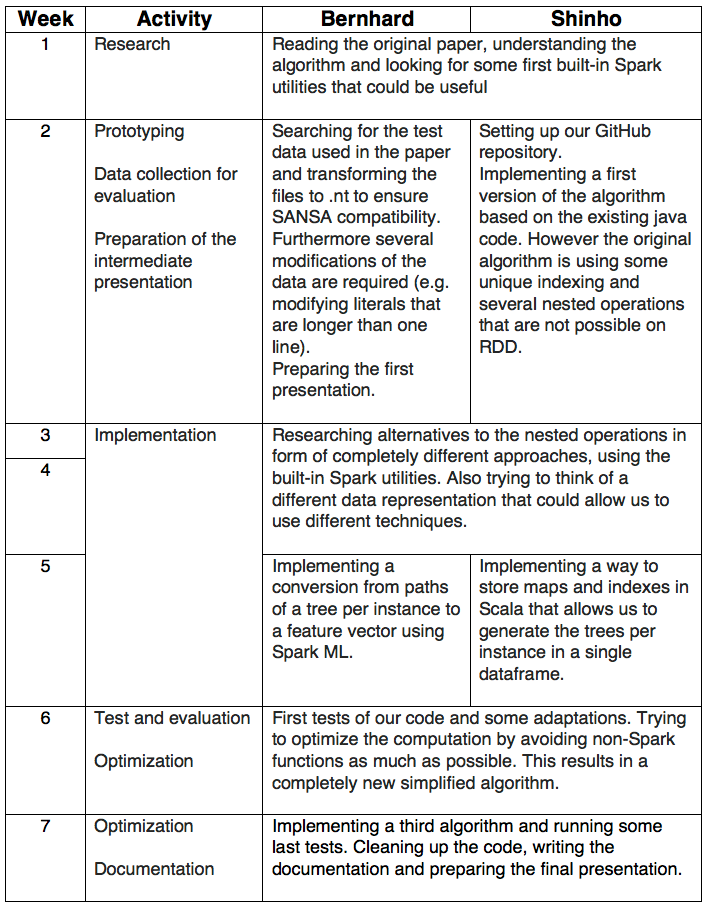
\includegraphics[width=14cm]{Timeline.png}

\subsection{Further ideas}
Up until now the algorithms have only been tested locally with medium size data files. The next step would be tests with bigger data on a real cluster with different nodes to see how the different algorithms perform under those conditions. While the basic RDFFastTreeGraphKernel will probably struggle with long initialization times, the other two alternatives should be quite performant. Furthermore it would be interesting to see how different learning algorithms like SVM or neural networks deal with the feature vectors generated by our kernels. Maybe the sparsity of our feature vectors can be further exploited.

%------------------------------------------------------------------------------


%------------------------------------------------------------------------------
% Refs:
%
\label{sect:bib}
\bibliographystyle{plain}
%\bibliographystyle{alpha}
%\bibliographystyle{unsrt}
%\bibliographystyle{abbrv}
\bibliography{fast_graph_kernel}

%------------------------------------------------------------------------------
% Index
%\printindex

%------------------------------------------------------------------------------
\end{document}

% EOF
